\appendix

\chapter{Computation of localized sets}
For each basic block there are 3 bit vectors dedicated to the block-specific
properties, namely \texttt{Transp}, \texttt{Antloc} and \texttt{Xcomp}. As
mentioned before, a bit vector is a boolean array of value numbers.  Let the
leader expression (as defined in the section on value numbering) associated
with the value number $v$ be called $L(v)$. 


\begin{equation}
\begin{array}{l c l}
\texttt{Transp(v,B)} &=& \left\{
                    \begin{array}{l l}
                        false & \quad \text{iff $\exists$ x $\in$ operands of L(v) such that \texttt{Mod(x,B)} = true}\\
                        true & \quad \text{Otherwise}
                    \end{array} \right. \\
\texttt{Antloc(v,B)} &=& \texttt{Eval(v,B)} \cap \texttt{Transp(v,B)} \\
\texttt{Xcomp(v,B)} &=& \texttt{Eval(v,B)} \cap \overline{\texttt{Transp(v,B)}}\\
  &&\\
\text{where}&& \\  
\quad \texttt{Eval(v,B)} &=& \text{\{v $|$ value number v is computed in B\}}\\
\quad \texttt{Mod(op,B)} &=& \text{operand op modified in B}\\
\end{array}
\end{equation}

\chapter{Lazy Code motion Transformations}

\begin{itemize}
\item Down Safety Analysis (Backward data flow analysis)
\begin{equation}
\begin{array}{l c l}
\antin{b} &=& \antloc{b} \cup (\transp{b} \cap \antout{b}) \\
\antout{b} &=& \xcomp{b} \cup \left\{
                    \begin{array}{l l}
                        \phi & \quad \text{if b = exit}\\
                        \displaystyle \bigcap_{s \in succ(b)} \antin{s} &
                    \end{array} \right. \\
\end{array}
\end{equation}

\item Up Safety Analysis (Forward data flow analysis)
\begin{equation}
\begin{array}{l c l}
\availin{b} &=& \left\{
                  \begin{array}{l l}
                        \phi & \quad \text{if b = entry}\\
                        \displaystyle \bigcap_{p \in pred(b)} (\xcomp{p} \cup \availout{p}) & 
                  \end{array} 
              \right. \\
\availout{b} &=& \transp{b} \cap (\antloc{b} \cup \availin{b}) \\
\end{array}
\end{equation}

\item Earliest-ness (No data flow analysis)
\begin{equation}
\begin{array}{l c l}
\earlin{b}  &=& \antin{b} \cap \displaystyle \bigcap_{p \in pred(b)} (\overline{\availout{p} \cup \antout{p}}) \\ 
\earlout{b} &=& \antout{b} \cap \overline{\transp{b}}
\end{array}
\end{equation}

\item Delayability (Forward data flow analysis)
\begin{equation}
\begin{array}{l c l}
\delayin{b} &=& \earlin{b} \cup  \left\{
                              \begin{array}{l l}
                                \phi & \quad \text{if b = entry}\\
                                \displaystyle \bigcap_{p \in pred(b)} (\overline{\xcomp{p}} \cap \delayout{p}) & 
                  \end{array} 
              \right. \\
\delayout{b} &=& \earlout{b} \cup (\delayin{b} \cap \overline{\antloc{b}}) \\
\end{array}
\end{equation}

\item Latest-ness (No data flow analysis)
\begin{equation}
\begin{array}{l c l}
\latestin{b}  &=& \delayin{b} \cap \antloc{b}\\
\latestout{b} &=& \delayout{b} \cap (\xcomp{b} \cup \displaystyle \bigcup_{s \in succ(b)} \overline{\delayin{s}})
\end{array}
\end{equation}


\item Isolation Analysis (Backward data flow analysis)
\begin{equation}
\begin{array}{l c l}
\isoin{b} &=& \earlout{b} \cup \isoout{b} \\
\isoout{b} &=& \left\{
                    \begin{array}{l l}
                        U & \quad \text{if b = exit}\\
                        \displaystyle \bigcap_{s \in succ(b)} (\earlin{s} \cup (\overline{\antloc{s}} \cap \isoin{s}) )&
                    \end{array} \right. \\
\end{array}
\end{equation}

\item Insert and Replace points
\begin{equation}
\begin{array}{l c l}
\insertin{b} &=& \latestin{b} \cap \overline{\isoin{b}} \\
\insertout{b} &=& \latestout{b} \cap \overline{\isoout{b}} \\
&&\\
\replacein{b} &=& \antloc{b} \cap \overline{\latestin{b} \cap \isoin{b}} \\
\replaceout{b} &=& \xcomp{b} \cap \overline{\latestout{b} \cap \isoout{b}}
\end{array}
\end{equation}
\end{itemize}

\chapter{Generalized data flow framework}

All the equations in Appendix B can be computed using the generic
framework defined below.

\section{Forward Analysis}
\begin{equation}
\begin{array}{l c l}
\myin{b} &=& \Alpha{b} \cup  \left\{
                    \begin{array}{l l}
                        \bot & \quad \text{if b = entry}\\
                        \displaystyle \bigwedge_{p \in pred(b)} \Beta{p}&
                    \end{array} \right. \\
\myout{b} &=& \myGamma{b}                      
\end{array}
\end{equation}

\section{Backward Analysis}
\begin{equation}
\begin{array}{l c l}
\myin{b} &=& \myGamma{b}                      \\
\myout{b} &=& \Alpha{b} \cup  \left\{
                    \begin{array}{l l}
                        \bot & \quad \text{if b = exit}\\
                        \displaystyle \bigwedge_{s \in succ(b)} \Beta{s}&
                    \end{array} \right. \\
\end{array}
\end{equation}

The following is the function which we call with dataflow equation
specific parameters defined subsequently.

\begin{framed}
\[
\texttt{callFramework}(\myout{b}, \myin{b}, \Alpha{b}, \Beta{b},\myGamma{b}, \bigwedge, \bot, \top, \text{Direction})
\]
\end{framed}

Following is the list of values that we need to plug-in to $\alpha$,
          $\beta$ and $\gamma$ for the above generic framework
          to work.



\begin{itemize}
\item Down Safety Analysis (Backward data flow analysis)
\begin{equation}
\begin{array}{l c l}
\Alpha{x}     &=& \xcomp{x} \\
\Beta{x}      &=& \antin{x}     \\     
\myGamma{x}   &=& \transp{x} \cap \antout{x} \cup \antloc{x}\\
\bigwedge     &=&  \cap \\
\bot          &=& \phi \\
\top          &=& V, \text{set of all values} \\
\text{Direction}    &=& \text{Backward}
\end{array}
\end{equation}

\item Up Safety Analysis (Forward data flow analysis)
\begin{equation}
\begin{array}{l c l}
\Beta{x}      &=& \xcomp{x} \cup \availout{x}     \\     
\myGamma{x}   &=& \antloc{x} \cup \availin{x} \cap \transp{x}\\
\bigwedge     &=&  \cap \\
\bot          &=& \phi \\
\top          &=& V, \text{set of all values} \\
\text{Direction}    &=& \text{Forward}
\end{array}
\end{equation}

\item Delayability (Forward data flow analysis)
\begin{equation}
\begin{array}{l c l}
\Alpha{x}     &=& \earlin{x} \\
\Beta{x}      &=& \overline{\xcomp{x}} \cap \delayout{x}     \\     
\myGamma{x}   &=& \delayin{x} \cap \overline{\antloc{x}} \cup \earlout{x}\\
\bigwedge     &=&  \cap \\
\bot          &=& \phi \\
\top          &=& V, \text{set of all values} \\
\text{Direction}    &=& \text{Forward}
\end{array}
\end{equation}

\item Isolation Analysis (Backward data flow analysis)
\begin{equation}
\begin{array}{l c l}
\Beta{x}      &=& \overline{\antloc{x}} \cap \isoin{x} \cup \earlin{x}     \\     
\myGamma{x}   &=& \earlout{x} \cup \isoout{x} \\
\bigwedge     &=&  \cap \\
\bot          &=& V, \text{set of all values} \\
\top          &=& V, \text{set of all values} \\
\text{Direction}    &=& \text{Backward}
\end{array}
\end{equation}

\end{itemize}

\chapter{Transformations for ``Zero-trip Loops''}

\begin{figure}[htbp]
  \begin{center}
     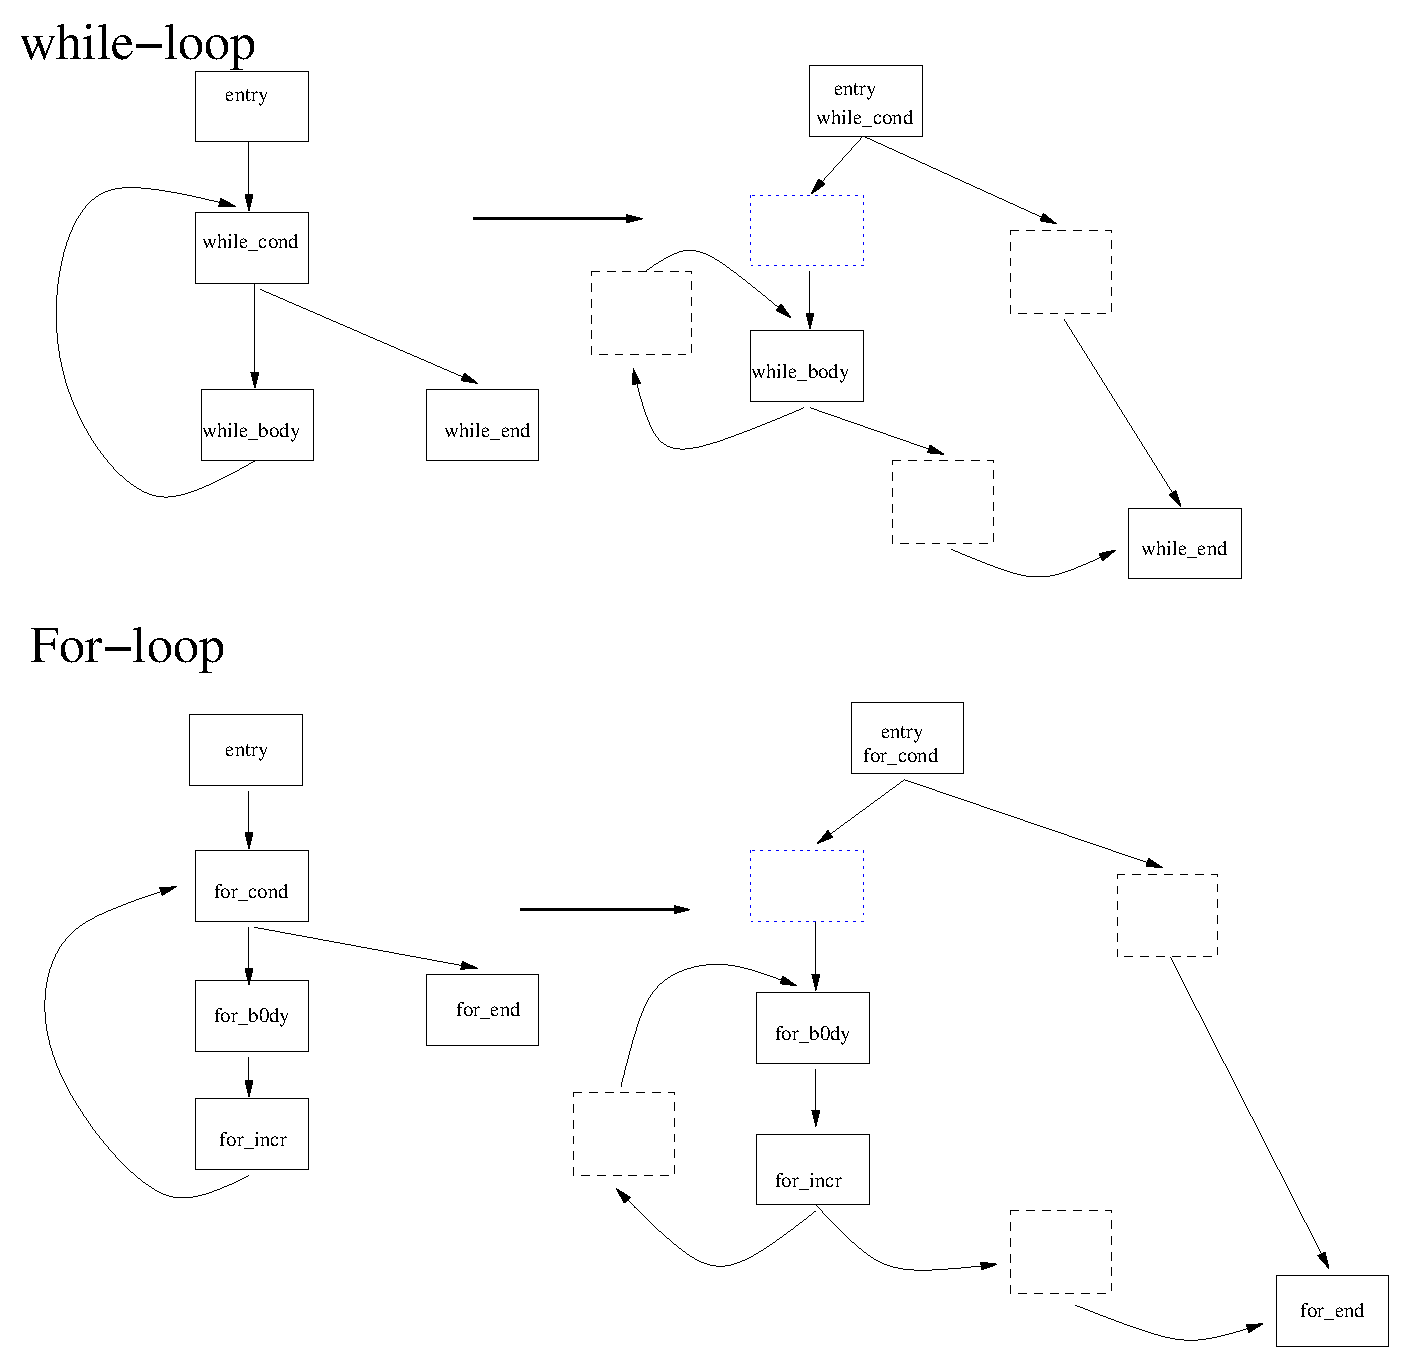
\includegraphics[scale=0.5]{Figs/5} 
  \end{center}
  \caption{Loop transformations done by \emph{-loop-rotate}. \emph{do-while}
    loops remain unaffected. Blue dotted boxes are the ones inserted by loop
      rotate. PRE can insert the computations in these places.}
  \label{fig:5} 
  \end{figure}


\chapter{An Extended Example}

Here we show, through an example code, the optimizations performed
by our PRE pass. The intention here is to highlight redundancy elimination for  
expressions $a + b$ \& $a < b$. Optimal placements are marked in Figure \ref{fig:2}.
Some of the notable obseravtions are:
\begin{itemize}
\item Black dotted boxes denote basic blocks inserted because of critical edge splitting
\item  Blue dotted boxes are the loop pre-headers inserted
      by -loop-rotate pass. PRE can insert computations here.
\item Inserted statements are marked \textcolor{blue}{blue} and replaced ones with
      \textcolor{magenta}{magenta}      
\item LCSE (Local common subexpression elimination)  happened in BB2.
\item For the loop {BB7,BB9} in Figure \ref{fig:1}, LICM happened wherein the computation 
of $a+b$ is moved from BB9 (in Figure  \ref{fig:1}) to BB8 (in Figure \ref{fig:2}). BB8 is the loop pre-header
\end{itemize}


\begin{figure}[htbp]
  \begin{center}
     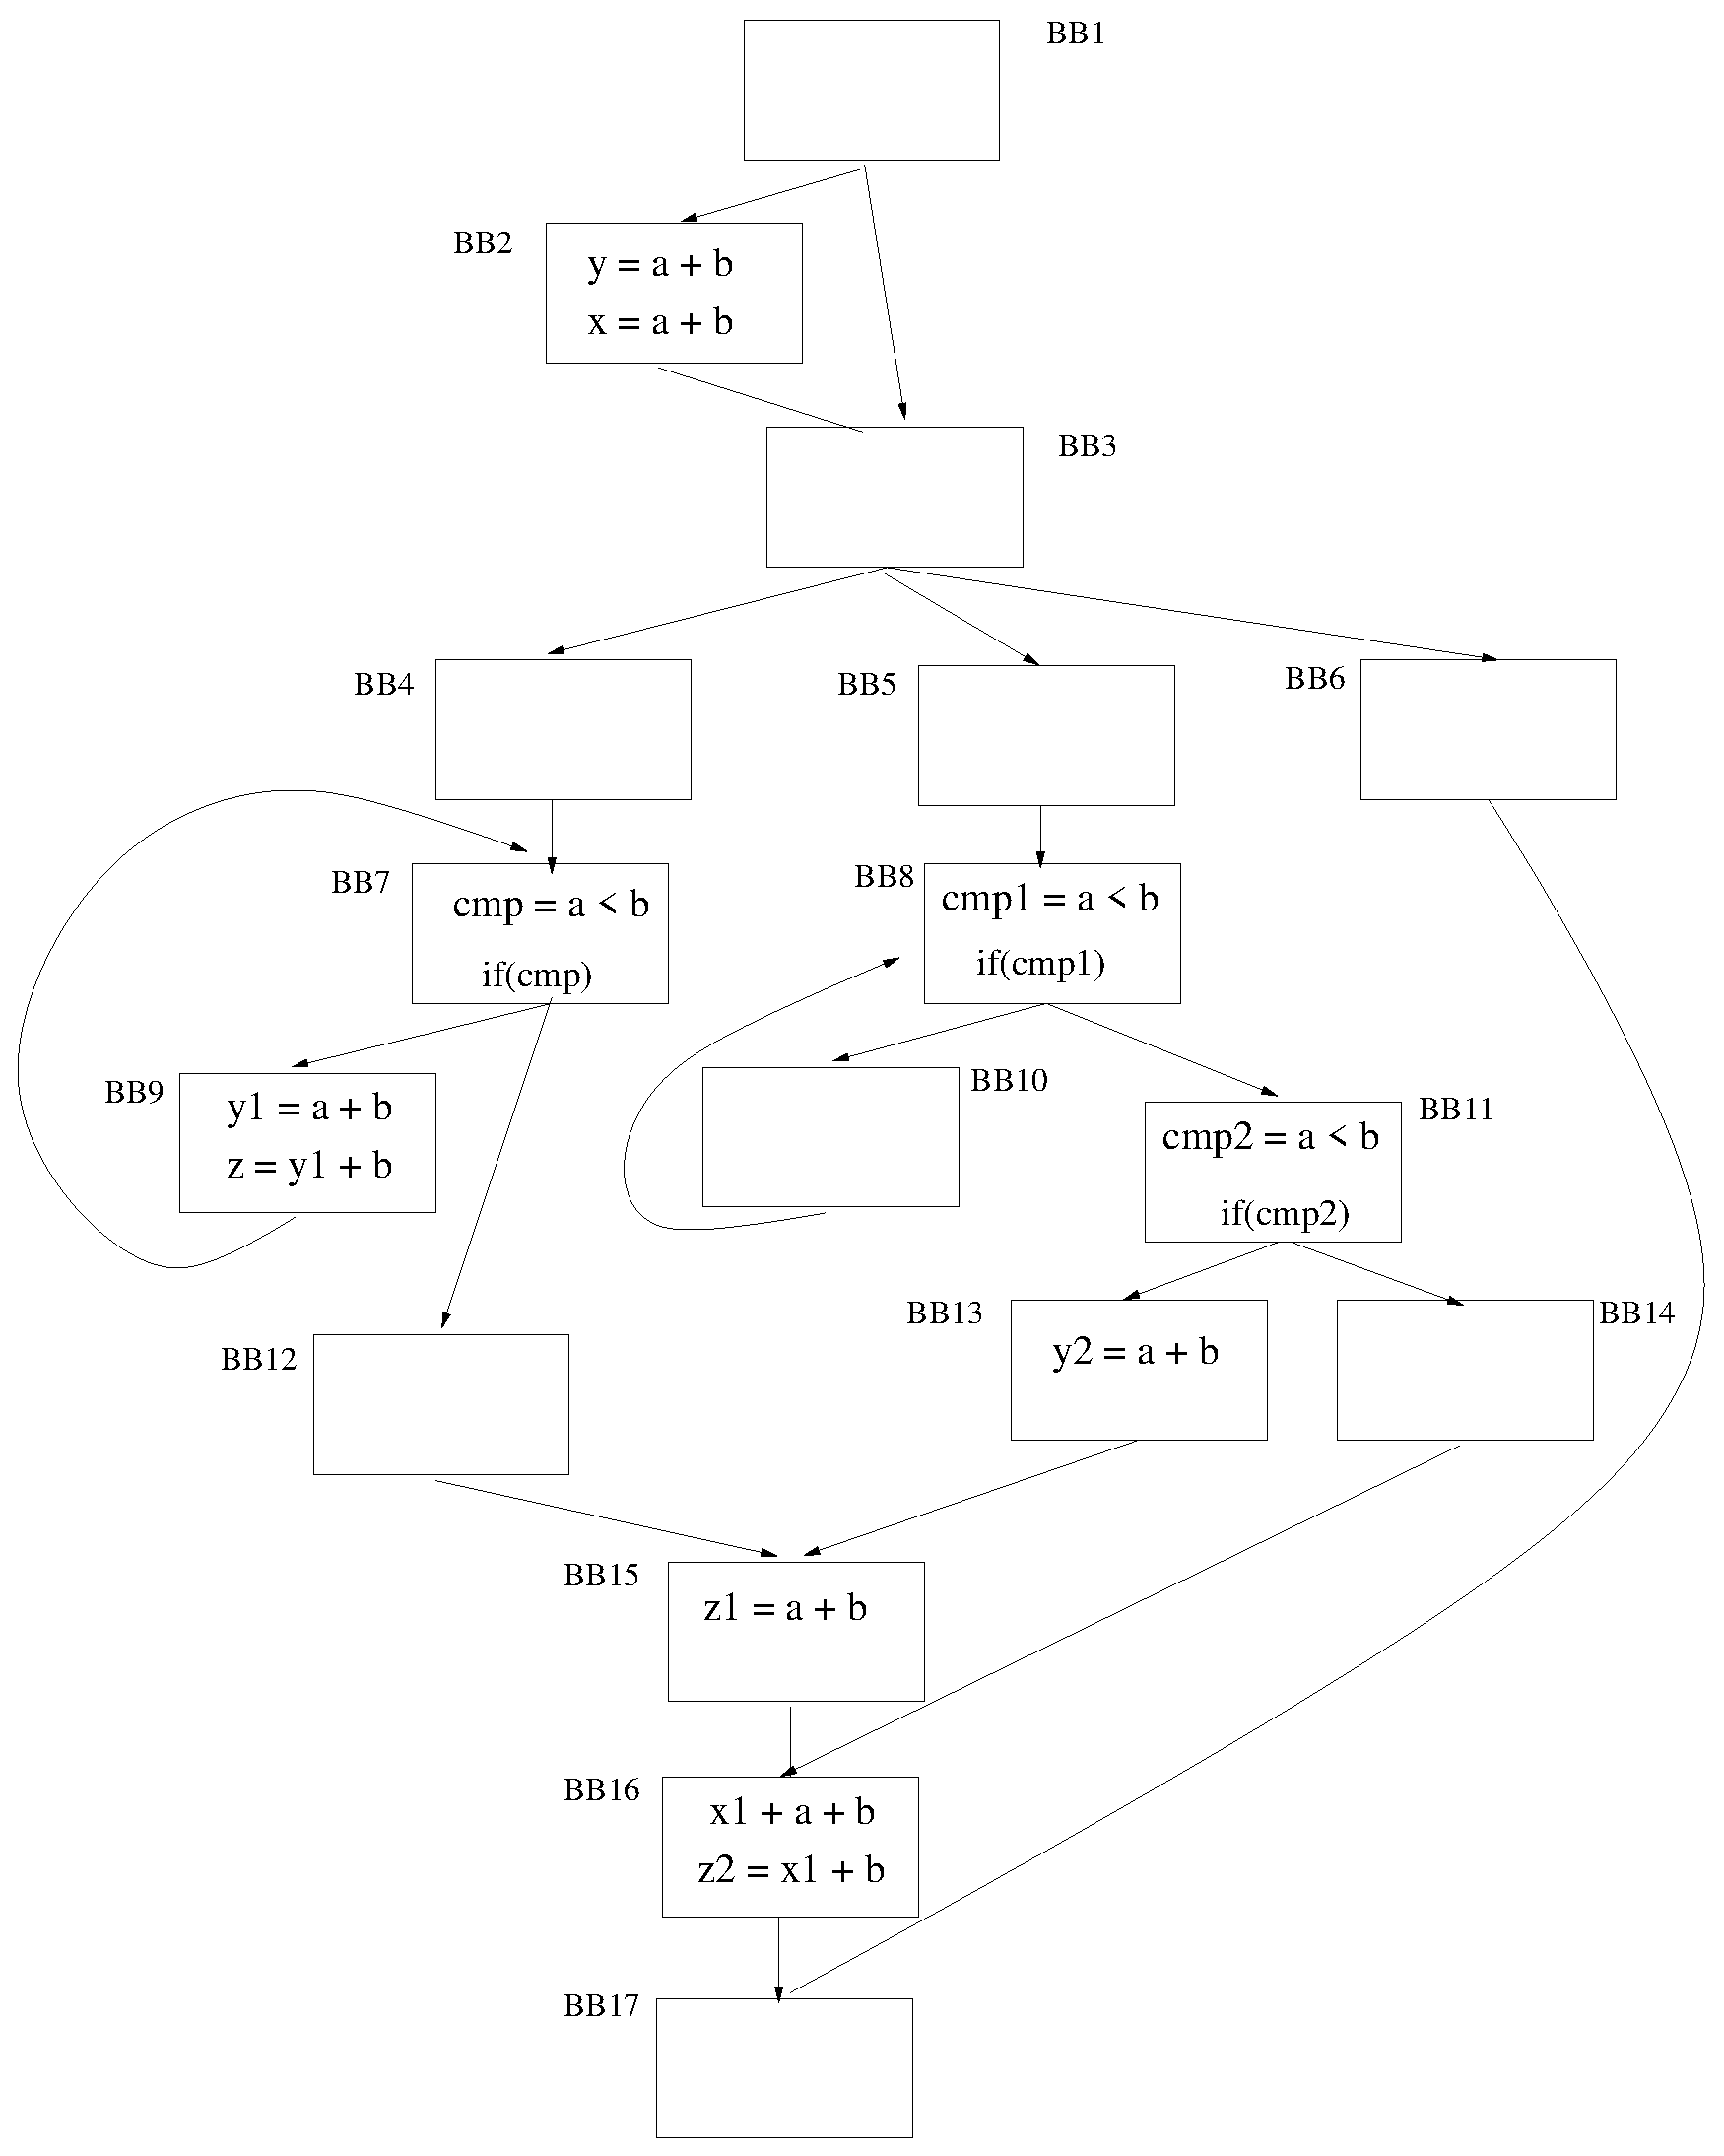
\includegraphics[scale=0.3]{Figs/1} 
  \end{center}
  \caption{A motivating example}
    \label{fig:1} 
\end{figure}

\begin{figure}[htbp]
  \begin{center}
     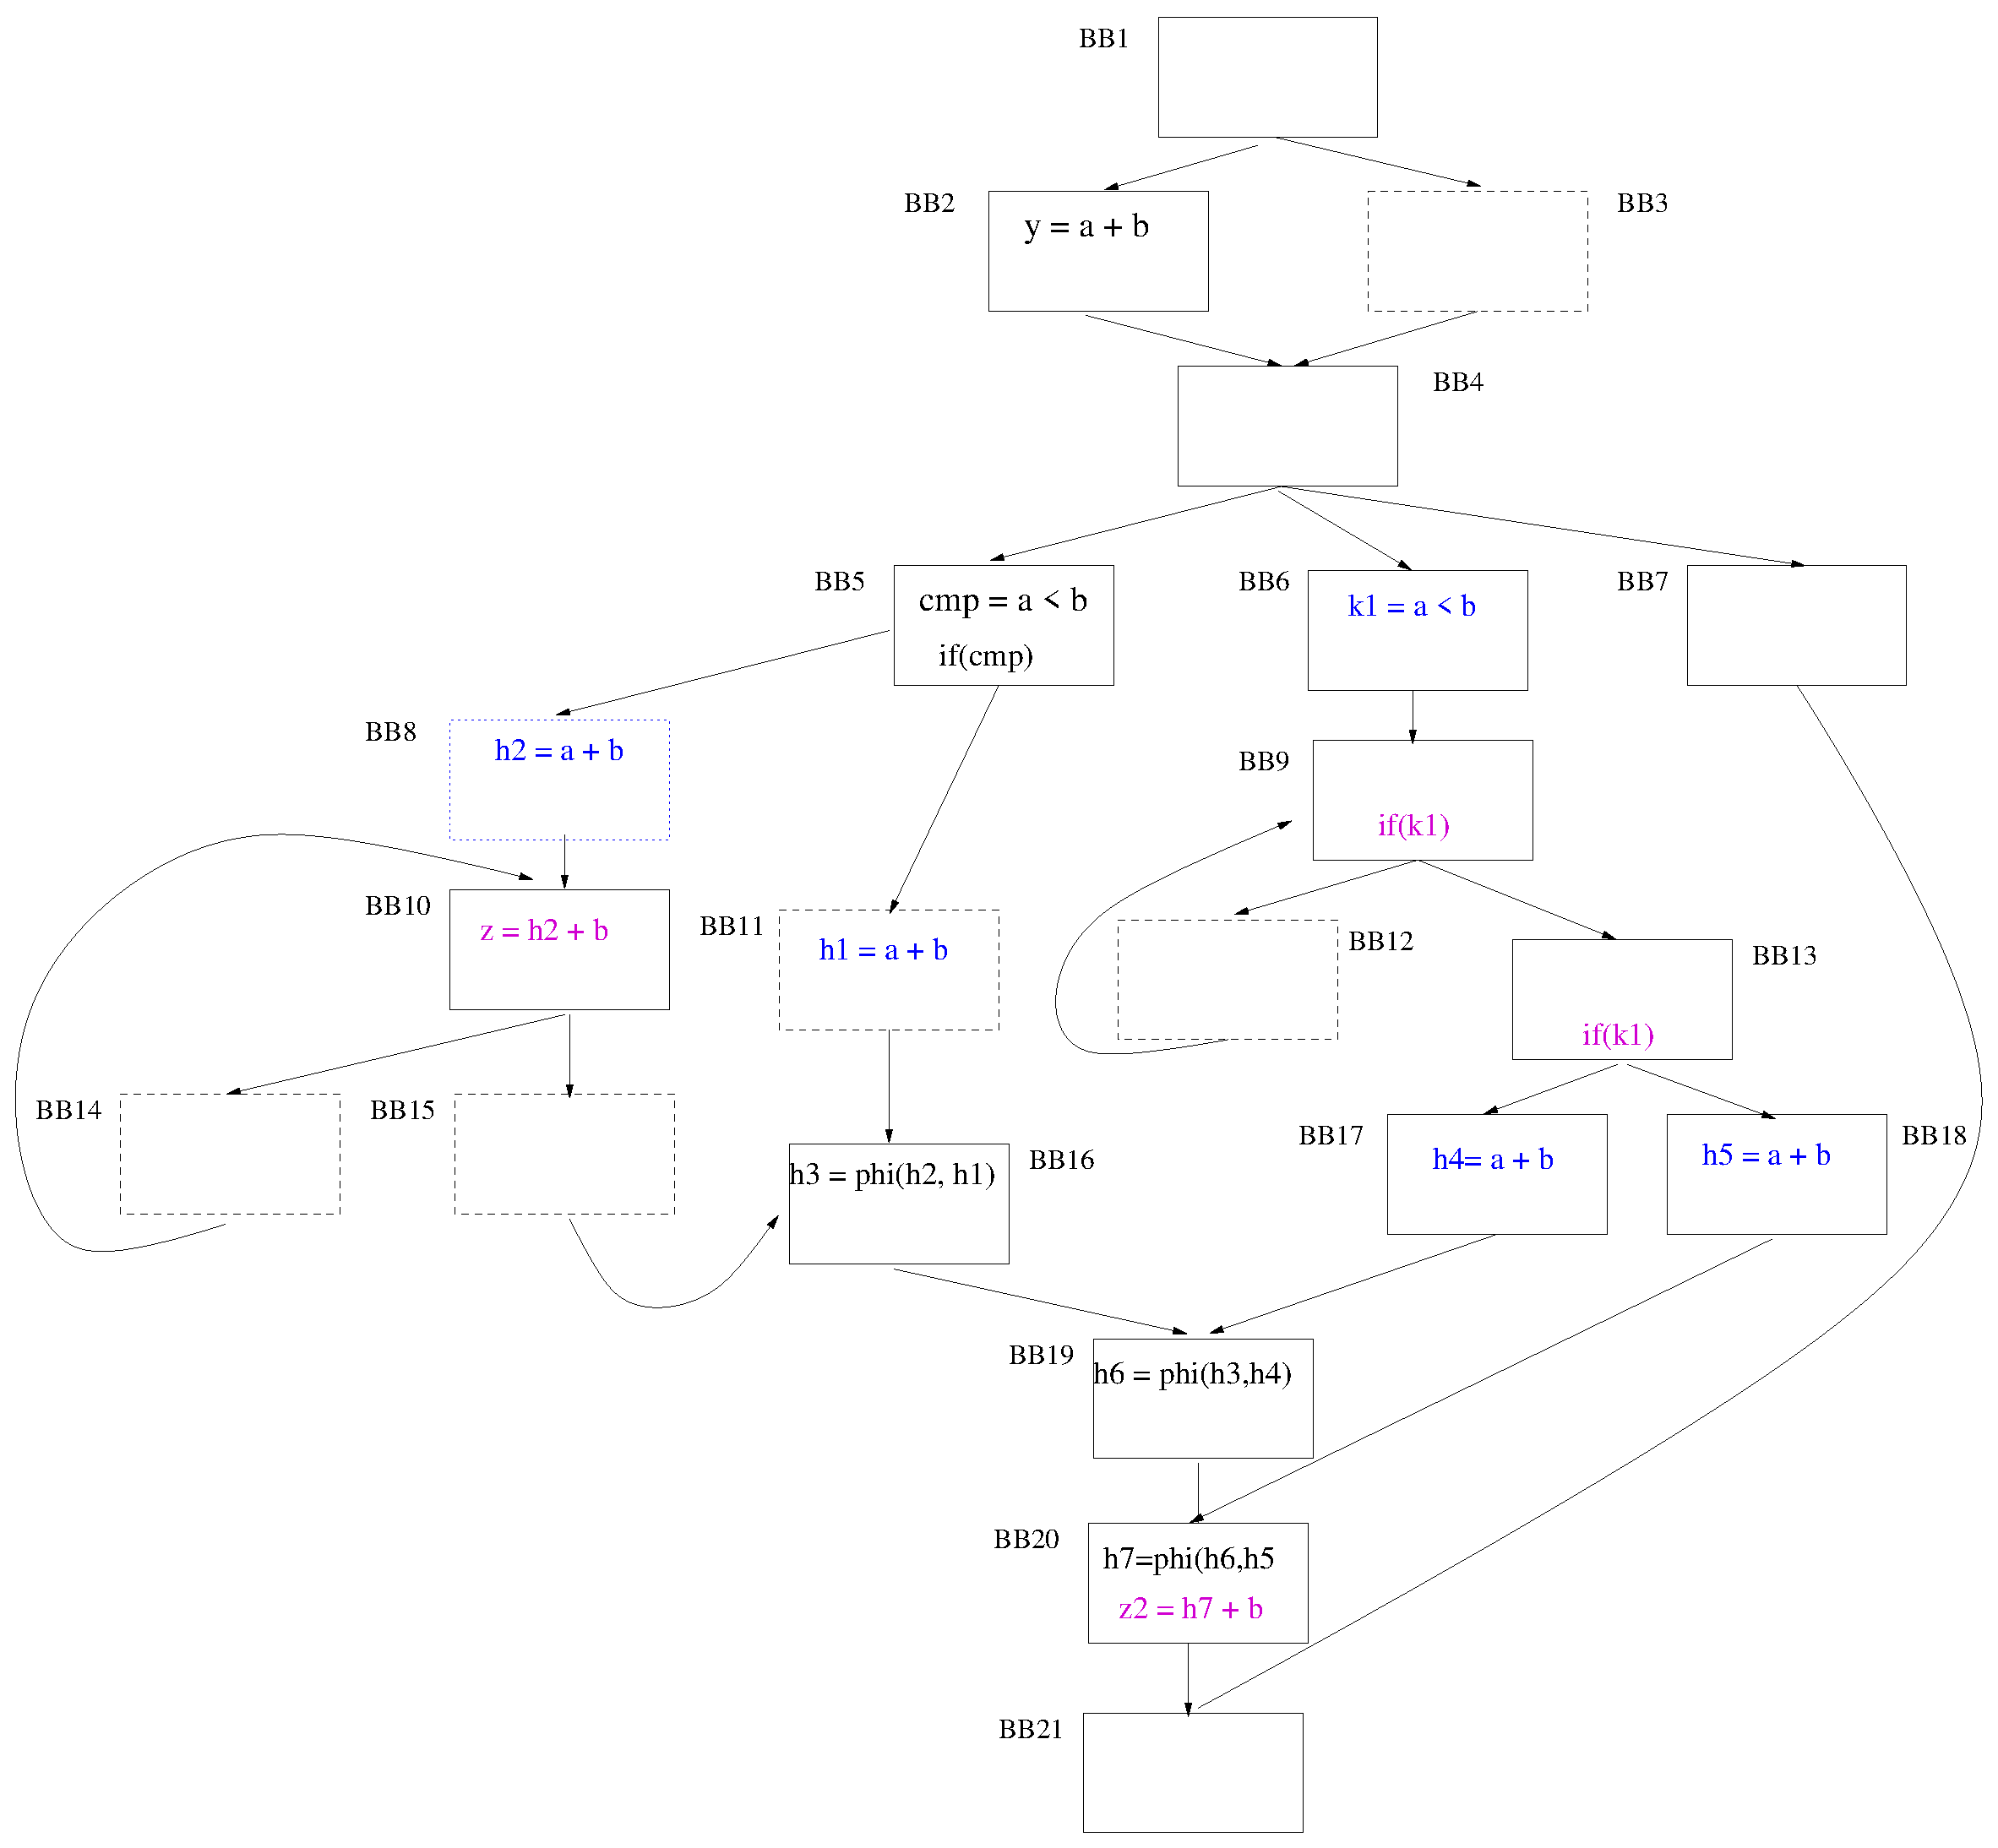
\includegraphics[scale=0.3]{Figs/2} 
  \end{center}
  \caption{Lazy code motion transformation on computations $a + b$ \& $a < b$.}
  \label{fig:2} 
\end{figure}
